\item \textbf{{[}ACJC/PRELIM/9569/2021/P2/Q2{]} }

\noindent A file compression algorithm reduces file sizes so that
files can be sent more quickly. One such algorithm is the Huffman
algorithm for text files, which will be implemented in this task.

\noindent Unlike ASCII, which assigns a fixed size of 8 bits for each
character, the Huffman algorithm assigns fewer bits to more common
characters and more bits to less common characters. For example, in
a long text written in English, characters such as '\texttt{e}' and
'\texttt{t}' will have fewer bits assigned to them than characters
such as '\texttt{q}' and '\texttt{z}'. If the text is long enough,
this will use fewer bits in total to encode the text compared to ASCII.

\noindent To know which sequence of bits to encode for each character,
the \textbf{frequency} of each character, which is the number of times
each character appears in the text file, is tabulated.

\noindent The characters are put into a tree. A node is created for
each character. The following steps are then repeated until there
is only one node without a parent:
\begin{enumerate}
\item Identify the two nodes, without parents, which have the lowest frequency. 
\item Create a new node whose left and right children are the two nodes
identified in Step 1. The frequency of the new node is the total of
the frequency of its children.
\end{enumerate}
\noindent The diagram on the following page shows the process of creation
of a tree for a file with only five distinct characters ('\texttt{A}',
'\texttt{E}', '\texttt{I}', '\texttt{O}' and '\texttt{U}'), in five
stages.

\noindent The bit sequence assigned to a character will be the path
from the root to the node corresponding to that character, where going
left corresponds to '\texttt{0}' and going right corresponds to '\texttt{1}'.
For example, '\texttt{A}' is encoded as '\texttt{10}' and '\texttt{O}'
is encoded as '\texttt{011}'.

\subsection*{Task 2.1}

\noindent Create a Node class that has the following attributes: 
\begin{itemize}
\item \texttt{data}, which is determined when the node is initialized 
\item \texttt{left}, a pointer to another node, 
\item \texttt{right}, a pointer to another node 
\end{itemize}
\noindent When the node is initialised, left and right do not point
to anything. The class also has setter methods for left and right,
and getter methods for all three attributes. \hfill{}{[}3{]}

\subsection*{Task 2.2}

\noindent Write code that takes an input \texttt{.txt} file and creates
a dictionary whose keys are the characters in the file, including
spaces, punctuation and line breaks ('\texttt{\textbackslash n}'),
and the value of a key is its frequency in the file. Uppercase and
lowercase letters should be considered as different characters.

\noindent Create a node for each character in the file, and put the
nodes into a list in ascending order of frequency. \hfill{}{[}11{]}

\subsection*{Task 2.3}

\noindent Create a tree using the algorithm described above. \hfill{}{[}5{]}

\subsection*{Task 2.4}

\noindent Create a dictionary whose keys are the characters, and the
value of a key is the bit sequence of that character, expressed as
a string of '\texttt{0}'s and '\texttt{1}'s.

\noindent Carry out Tasks 2.2 to 2.4 on the file \texttt{HAMLET.txt}.
Compress the file by replacing each character with its bit sequence
and writing the output to a new file, \texttt{HAMLET\_compressed.txt}.
{[}8{]}

\noindent Download your program code and output for Task 2 as \texttt{TASK2\_<your
name>\_<centre number>\_<index number>.ipynb} 

\noindent Diagram showing how the tree is created based on the frequency
of each character: 
\noindent \begin{center}
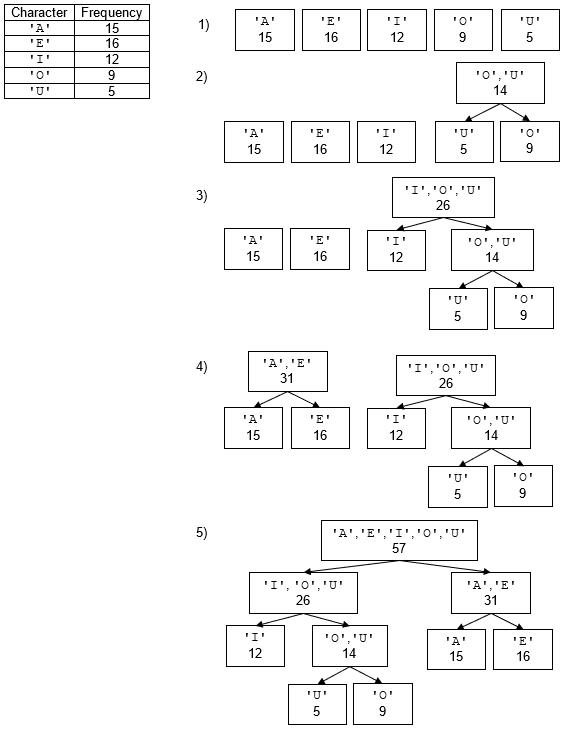
\includegraphics[scale=0.8]{C:/Users/Admin/Desktop/Github/question_bank/LyX/static/img/9569-ACJC-2021-P2-Q2}\quad{}
\par\end{center}